\documentclass[../report.tex]{subfiles}

\begin{document}

\subsection{CRC}
\renewcommand{\arraystretch}{1.5}

{\bfseries\Large Book} \\
\begin{tabular}{| m{8cm} | m{3cm} | m{5.5cm} |}
\hline
\multicolumn{3}{|c|}{\textbf{Front}} \\
\hline
\textbf{Tên lớp}: Book & \textbf{ID}: 1 & \textbf{Loại}: Cụ thể \\
\hline
\multicolumn{2}{|l|}{\textbf{Mô tả}: Chứa thông tin từng cuốn sách} & \textbf{Ca sử dụng được liên kết}: \\
\hline
\multicolumn{1}{|c}{\textbf{Nhiệm vụ}} & 
\multicolumn{2}{|c|}{\textbf{Cộng tác}} \\
\hline
\tabitem Lấy thông tin tiêu đề sách & \multicolumn{2}{l|}{\tabitem BookTitle} \\
\tabitem Lấy thông tin về nhóm ngành & \multicolumn{2}{l|}{\tabitem Topic} \\
\tabitem Lấy ID & \multicolumn{2}{l|}{} \\
\tabitem Lấy trạng thái của sách: được phép mượn hoặc không được mượn (chỉ đọc) & \multicolumn{2}{l|}{} \\

\hline
\end{tabular} \\[1cm]
\begin{tabular}{| m{8.5cm} | m{8.5cm} |}
\hline
\multicolumn{2}{|c|}{\textbf{Back}} \\
\hline
\multicolumn{2}{|l|}{\textbf{Thuộc tính:}} \\
\hline
\multicolumn{2}{|l|}{1. bookID} \\
\multicolumn{2}{|l|}{2. bookTitle} \\
\multicolumn{2}{|l|}{3. allowBorrow} \\
\hline
\textbf{Quan hệ}: & \\
\tabitem Kế thừa (a-kind-of): & \\
\tabitem Kết tập (has-parts): BookTitle & \\
\tabitem Liên kết: & \\
\hline
\end{tabular}\\[1cm]

\newpage
{\bfseries\Large BookTitle} \\[0.3cm]
\begin{tabular}{| m{8cm} | m{3cm} | m{5.5cm} |}
\hline
\multicolumn{3}{|c|}{\textbf{Front}} \\
\hline
\textbf{Tên lớp}: BookTitle & \textbf{ID}: 2 & \textbf{Loại}: Cụ thể \\
\hline
\multicolumn{2}{|l|}{\textbf{Mô tả}: Chứa thông tin về tên sách và nhóm ngành} & \textbf{Ca sử dụng được liên kết}: \\
\hline
\multicolumn{1}{|c}{\textbf{Nhiệm vụ}} & 
\multicolumn{2}{|c|}{\textbf{Cộng tác}} \\
\hline
\tabitem Lấy thông tin tên sách, NXB, tác giả, năm xuất bản, giá sách & \multicolumn{2}{l|}{\tabitem Topic} \\
\tabitem Lấy thông tin về nhóm ngành & \multicolumn{2}{l|}{\tabitem Book} \\
\tabitem Lấy ID & \multicolumn{2}{l|}{} \\
\hline
\end{tabular} \\[1cm]
\begin{tabular}{| m{8.5cm} | m{8.5cm} |}
\hline
\multicolumn{2}{|c|}{\textbf{Back}} \\
\hline
\multicolumn{2}{|l|}{\textbf{Thuộc tính:}} \\
\hline
\multicolumn{2}{|l|}{1. bookTitleID} \\
\multicolumn{2}{|l|}{2. name} \\
\multicolumn{2}{|l|}{3. publisher} \\
\multicolumn{2}{|l|}{4. publishYear} \\
\multicolumn{2}{|l|}{5. author} \\
\multicolumn{2}{|l|}{6. price} \\
\multicolumn{2}{|l|}{7. topic} \\
\hline
\textbf{Quan hệ}: & \\
\tabitem Kế thừa (a-kind-of): & \\
\tabitem Kết tập (has-parts): Topic & \\
\tabitem Liên kết: & \\
\hline
\end{tabular}\\[1cm]

\newpage
{\bfseries\Large Topic} \\[0.3cm]
\begin{tabular}{| m{8cm} | m{3cm} | m{5.5cm} |}
\hline
\multicolumn{3}{|c|}{\textbf{Front}} \\
\hline
\textbf{Tên lớp}: Topic & \textbf{ID}: 3 & \textbf{Loại}: Cụ thể \\
\hline
\multicolumn{2}{|l|}{\textbf{Mô tả}: Chứa thông tin về nhóm ngành} & \textbf{Ca sử dụng được liên kết}: \\
\hline
\multicolumn{1}{|c}{\textbf{Nhiệm vụ}} & 
\multicolumn{2}{|c|}{\textbf{Cộng tác}} \\
\hline
\tabitem Lấy tên nhóm ngành & \multicolumn{2}{l|}{} \\
\tabitem Lấy ID & \multicolumn{2}{l|}{} \\
\hline
\end{tabular} \\[1cm]
\begin{tabular}{| m{8.5cm} | m{8.5cm} |}
\hline
\multicolumn{2}{|c|}{\textbf{Back}} \\
\hline
\multicolumn{2}{|l|}{\textbf{Thuộc tính:}} \\
\hline
\multicolumn{2}{|l|}{1. topicID} \\
\multicolumn{2}{|l|}{2. name} \\
\hline
\textbf{Quan hệ}: & \\
\tabitem Kế thừa (a-kind-of): & \\
\tabitem Kết tập (has-parts): & \\
\tabitem Liên kết: & \\
\hline
\end{tabular}\\[1cm]

{\bfseries\Large Account} \\[0.3cm]
\begin{tabular}{| m{8cm} | m{3cm} | m{5.5cm} |}
\hline
\multicolumn{3}{|c|}{\textbf{Front}} \\
\hline
\textbf{Tên lớp}: Account & \textbf{ID}: 4 & \textbf{Loại}: Cụ thể \\
\hline
\multicolumn{2}{|l|}{\textbf{Mô tả}: Chứa thông tin tài khoản người dùng} & \textbf{Ca sử dụng được liên kết}: \\
\hline
\multicolumn{1}{|c}{\textbf{Nhiệm vụ}} & 
\multicolumn{2}{|c|}{\textbf{Cộng tác}} \\
\hline
\tabitem Lấy tên người dùng & \multicolumn{2}{l|}{} \\
\tabitem Lấy ID & \multicolumn{2}{l|}{} \\
\tabitem Lấy quyền của tài khoản & \multicolumn{2}{l|}{\tabitem Privilege} \\
\hline
\end{tabular} \\[1cm]
\begin{tabular}{| m{8.5cm} | m{8.5cm} |}
\hline
\multicolumn{2}{|c|}{\textbf{Back}} \\
\hline
\multicolumn{2}{|l|}{\textbf{Thuộc tính:}} \\
\hline
\multicolumn{2}{|l|}{1. accountID} \\
\multicolumn{2}{|l|}{2. name} \\
\multicolumn{2}{|l|}{3. email} \\
\multicolumn{2}{|l|}{4. privilege} \\
\multicolumn{2}{|l|}{5. password} \\
\hline
\textbf{Quan hệ}: & \\
\tabitem Kế thừa (a-kind-of): & \\
\tabitem Kết tập (has-parts): Privilege & \\
\tabitem Liên kết: & \\
\hline
\end{tabular}\\[1cm]

{\bfseries\Large Privilege} \\[0.3cm]
\begin{tabular}{| m{8cm} | m{3cm} | m{5.5cm} |}
\hline
\multicolumn{3}{|c|}{\textbf{Front}} \\
\hline
\textbf{Tên lớp}: Privilege & \textbf{ID}: 5 & \textbf{Loại}: Cụ thể \\
\hline
\multicolumn{2}{|l|}{\textbf{Mô tả}: Chứa thông tin quyền của tài khoản} & \textbf{Ca sử dụng được liên kết}: \\
\hline
\multicolumn{1}{|c}{\textbf{Nhiệm vụ}} & 
\multicolumn{2}{|c|}{\textbf{Cộng tác}} \\
\hline
\tabitem Lấy tên quyền & \multicolumn{2}{l|}{} \\
\tabitem Lấy ID quyền & \multicolumn{2}{l|}{} \\
\hline
\end{tabular} \\[1cm]
\begin{tabular}{| m{8.5cm} | m{8.5cm} |}
\hline
\multicolumn{2}{|c|}{\textbf{Back}} \\
\hline
\multicolumn{2}{|l|}{\textbf{Thuộc tính:}} \\
\hline
\multicolumn{2}{|l|}{1. privilegeID} \\
\multicolumn{2}{|l|}{2. name} \\
\hline
\textbf{Quan hệ}: & \\
\tabitem Kế thừa (a-kind-of): & \\
\tabitem Kết tập (has-parts): & \\
\tabitem Liên kết: & \\
\hline
\end{tabular}\\[1cm]

{\bfseries\Large Bill} \\[0.3cm]
\begin{tabular}{| m{8cm} | m{3cm} | m{5.5cm} |}
\hline
\multicolumn{3}{|c|}{\textbf{Front}} \\
\hline
\textbf{Tên lớp}: Bill & \textbf{ID}: 6 & \textbf{Loại}: Cụ thể \\
\hline
\multicolumn{2}{|l|}{\textbf{Mô tả}: Chứa thông tin một hóa đơn} & \textbf{Ca sử dụng được liên kết}: \\
\hline
\multicolumn{1}{|c}{\textbf{Nhiệm vụ}} & 
\multicolumn{2}{|c|}{\textbf{Cộng tác}} \\
\hline
\tabitem Lấy ngày mượn & \multicolumn{2}{l|}{} \\
\tabitem Lấy số tiền đặc cọc & \multicolumn{2}{l|}{} \\
\tabitem Lấy tài khoản tương ứng & \multicolumn{2}{l|}{\tabitem Account} \\
\tabitem Lấy sách trong hoá đơn & \multicolumn{2}{l|}{\tabitem Book} \\
\tabitem Lấy ID hóa đơn & \multicolumn{2}{l|}{} \\
\hline
\end{tabular} \\[1cm]
\begin{tabular}{| m{8.5cm} | m{8.5cm} |}
\hline
\multicolumn{2}{|c|}{\textbf{Back}} \\
\hline
\multicolumn{2}{|l|}{\textbf{Thuộc tính:}} \\
\hline
\multicolumn{2}{|l|}{1. billID} \\
\multicolumn{2}{|l|}{2. borrowedDate} \\
\multicolumn{2}{|l|}{3. deposit} \\
\multicolumn{2}{|l|}{4. account} \\
\multicolumn{2}{|l|}{5. books} \\
\hline
\textbf{Quan hệ}: & \\
\tabitem Kế thừa (a-kind-of): & \\
\tabitem Kết tập (has-parts): Account, Book & \\
\tabitem Liên kết: & \\
\hline
\end{tabular}\\[1cm]

{\bfseries\Large BookDAO} \\[0.3cm]
\begin{tabular}{| m{8cm} | m{3cm} | m{5.5cm} |}
\hline
\multicolumn{3}{|c|}{\textbf{Front}} \\
\hline
\textbf{Tên lớp}: BookDAO & \textbf{ID}: 7 & \textbf{Loại}: Cụ thể \\
\hline
\multicolumn{2}{|l|}{\textbf{Mô tả}: Interface cho tương tác với sách trong CSDL} & \textbf{Ca sử dụng được liên kết}: \\
\hline
\multicolumn{1}{|c}{\textbf{Nhiệm vụ}} & 
\multicolumn{2}{|c|}{\textbf{Cộng tác}} \\
\hline
\tabitem Tạo các sách & \multicolumn{2}{l|}{BookTitle} \\
\tabitem Xóa sách & \multicolumn{2}{l|}{} \\
\hline
\end{tabular} \\[1cm]
\begin{tabular}{| m{8.5cm} | m{8.5cm} |}
\hline
\multicolumn{2}{|c|}{\textbf{Back}} \\
\hline
\multicolumn{2}{|l|}{\textbf{Thuộc tính:}} \\
\hline
\textbf{Quan hệ}: & \\
\tabitem Kế thừa (a-kind-of): & \\
\tabitem Kết tập (has-parts): & \\
\tabitem Liên kết: BookTitle & \\
\hline
\end{tabular}\\[1cm]

{\bfseries\Large AccountDAO} \\[0.3cm]
\begin{tabular}{| m{8cm} | m{3cm} | m{5.5cm} |}
\hline
\multicolumn{3}{|c|}{\textbf{Front}} \\
\hline
\textbf{Tên lớp}: AccountDAO & \textbf{ID}: 8 & \textbf{Loại}: Cụ thể \\
\hline
\multicolumn{2}{|l|}{\textbf{Mô tả}: Interface thao tác với Tài khoản trong CSDL} & \textbf{Ca sử dụng được liên kết}: \\
\hline
\multicolumn{1}{|c}{\textbf{Nhiệm vụ}} & 
\multicolumn{2}{|c|}{\textbf{Cộng tác}} \\
\hline
\tabitem Lấy tài khoản từ CSDL & \multicolumn{2}{l|}{Account} \\
\tabitem Xóa tài khoản & \multicolumn{2}{l|}{} \\
\hline
\end{tabular} \\[1cm]
\begin{tabular}{| m{8.5cm} | m{8.5cm} |}
\hline
\multicolumn{2}{|c|}{\textbf{Back}} \\
\hline
\multicolumn{2}{|l|}{\textbf{Thuộc tính:}} \\
\hline
\textbf{Quan hệ}: & \\
\tabitem Kế thừa (a-kind-of): & \\
\tabitem Kết tập (has-parts): & \\
\tabitem Liên kết: Account & \\
\hline
\end{tabular}\\[1cm]

{\bfseries\Large BookTitleDAO} \\[0.3cm]
\begin{tabular}{| m{8cm} | m{3cm} | m{5.5cm} |}
\hline
\multicolumn{3}{|c|}{\textbf{Front}} \\
\hline
\textbf{Tên lớp}: BookTitleDAO & \textbf{ID}: 9 & \textbf{Loại}: Cụ thể \\
\hline
\multicolumn{2}{|l|}{\textbf{Mô tả}: Interface thao tác với Tiêu đề sách trong CSDL} & \textbf{Ca sử dụng được liên kết}: \\
\hline
\multicolumn{1}{|c}{\textbf{Nhiệm vụ}} & 
\multicolumn{2}{|c|}{\textbf{Cộng tác}} \\
\hline
\tabitem Thêm một tiêu đề sách & \multicolumn{2}{l|}{BookTitle} \\
\tabitem Xóa một tiêu đều sách & \multicolumn{2}{l|}{} \\
\tabitem Tìm kiếm theo tên & \multicolumn{2}{l|}{BookTitle} \\
\hline
\end{tabular} \\[1cm]
\begin{tabular}{| m{8.5cm} | m{8.5cm} |}
\hline
\multicolumn{2}{|c|}{\textbf{Back}} \\
\hline
\multicolumn{2}{|l|}{\textbf{Thuộc tính:}} \\
\hline
\textbf{Quan hệ}: & \\
\tabitem Kế thừa (a-kind-of): & \\
\tabitem Kết tập (has-parts): & \\
\tabitem Liên kết: BookTitle & \\
\hline
\end{tabular}\\[1cm]

{\bfseries\Large TopicDAO} \\[0.3cm]
\begin{tabular}{| m{8cm} | m{3cm} | m{5.5cm} |}
\hline
\multicolumn{3}{|c|}{\textbf{Front}} \\
\hline
\textbf{Tên lớp}: TopicDAO & \textbf{ID}: 10 & \textbf{Loại}: Cụ thể \\
\hline
\multicolumn{2}{|l|}{\textbf{Mô tả}: Interface thao tác với nhóm ngành trong CSDL} & \textbf{Ca sử dụng được liên kết}: \\
\hline
\multicolumn{1}{|c}{\textbf{Nhiệm vụ}} & 
\multicolumn{2}{|c|}{\textbf{Cộng tác}} \\
\hline
\tabitem Thêm một nhóm ngành & \multicolumn{2}{l|}{Topic} \\
\tabitem Xóa một nhóm ngành & \multicolumn{2}{l|}{} \\
\tabitem Lấy tất cả các nhóm ngành & \multicolumn{2}{l|}{Topic} \\
\hline
\end{tabular} \\[1cm]
\begin{tabular}{| m{8.5cm} | m{8.5cm} |}
\hline
\multicolumn{2}{|c|}{\textbf{Back}} \\
\hline
\multicolumn{2}{|l|}{\textbf{Thuộc tính:}} \\
\hline
\textbf{Quan hệ}: & \\
\tabitem Kế thừa (a-kind-of): & \\
\tabitem Kết tập (has-parts): & \\
\tabitem Liên kết: Topic & \\
\hline
\end{tabular}\\[1cm]

{\bfseries\Large BillDAO} \\[0.3cm]
\begin{tabular}{| m{8cm} | m{3cm} | m{5.5cm} |}
\hline
\multicolumn{3}{|c|}{\textbf{Front}} \\
\hline
\textbf{Tên lớp}: BillDAO & \textbf{ID}: 11 & \textbf{Loại}: Cụ thể \\
\hline
\multicolumn{2}{|l|}{\textbf{Mô tả}: Interface thao tác với hóa đơn trong CSDL} & \textbf{Ca sử dụng được liên kết}: \\
\hline
\multicolumn{1}{|c}{\textbf{Nhiệm vụ}} & 
\multicolumn{2}{|c|}{\textbf{Cộng tác}} \\
\hline
\tabitem Lấy các hóa đơn tương ứng với một tài khoản & \multicolumn{2}{l|}{Bill} \\
\tabitem Xóa một hóa đơn & \multicolumn{2}{l|}{} \\
\tabitem Thêm một hóa đơn & \multicolumn{2}{l|}{Bill} \\
\tabitem Trả một sách & \multicolumn{2}{l|}{} \\
\hline
\end{tabular} \\[1cm]
\begin{tabular}{| m{8.5cm} | m{8.5cm} |}
\hline
\multicolumn{2}{|c|}{\textbf{Back}} \\
\hline
\multicolumn{2}{|l|}{\textbf{Thuộc tính:}} \\
\hline
\textbf{Quan hệ}: & \\
\tabitem Kế thừa (a-kind-of): & \\
\tabitem Kết tập (has-parts): & \\
\tabitem Liên kết: Bill & \\
\hline
\end{tabular}\\[1cm]

{\bfseries\Large LoginController} \\[0.3cm]
\begin{tabular}{| m{8cm} | m{3cm} | m{5.5cm} |}
\hline
\multicolumn{3}{|c|}{\textbf{Front}} \\
\hline
\textbf{Tên lớp}: LoginController & \textbf{ID}: 12 & \textbf{Loại}: Cụ thể \\
\hline
\multicolumn{2}{|l|}{\textbf{Mô tả}: Đảm nhiệm chức năng đăng nhập} & \textbf{Ca sử dụng được liên kết}: Đăng nhập \\
\hline
\multicolumn{1}{|c}{\textbf{Nhiệm vụ}} & 
\multicolumn{2}{|c|}{\textbf{Cộng tác}} \\
\hline
\tabitem Đăng nhập & \multicolumn{2}{l|}{} \\
\hline
\end{tabular} \\[1cm]
\begin{tabular}{| m{8.5cm} | m{8.5cm} |}
\hline
\multicolumn{2}{|c|}{\textbf{Back}} \\
\hline
\multicolumn{2}{|l|}{\textbf{Thuộc tính:}} \\
\hline
\multicolumn{2}{|l|}{1. accountDAO} \\
\hline
\textbf{Quan hệ}: & \\
\tabitem Kế thừa (a-kind-of): & \\
\tabitem Kết tập (has-parts): AccountDAO& \\
\tabitem Liên kết: & \\
\hline
\end{tabular}\\[1cm]

{\bfseries\Large BookController} \\[0.3cm]
\begin{tabular}{| m{8cm} | m{3cm} | m{5.5cm} |}
\hline
\multicolumn{3}{|c|}{\textbf{Front}} \\
\hline
\textbf{Tên lớp}: BookController & \textbf{ID}: 13 & \textbf{Loại}: Cụ thể \\
\hline
\multicolumn{2}{|l|}{\textbf{Mô tả}: Đảm nhiệm chức năng liên quan tới sách} & \textbf{Ca sử dụng được liên kết}: Thêm tài liệu, Tra cứu sách, Báo mất sách \\
\hline
\multicolumn{1}{|c}{\textbf{Nhiệm vụ}} & 
\multicolumn{2}{|c|}{\textbf{Cộng tác}} \\
\hline
\tabitem Lấy danh sách các nhóm ngành & \multicolumn{2}{l|}{Topic} \\
\tabitem Thêm một nhóm ngành & \multicolumn{2}{l|}{Topic} \\
\tabitem Thêm một số lượng sách & \multicolumn{2}{l|}{BookTitle} \\
\tabitem Tìm kiếm sách & \multicolumn{2}{l|}{Book} \\
\tabitem Báo mất sách & \multicolumn{2}{l|}{} \\
\hline
\end{tabular} \\[1cm]
\begin{tabular}{| m{8.5cm} | m{8.5cm} |}
\hline
\multicolumn{2}{|c|}{\textbf{Back}} \\
\hline
\multicolumn{2}{|l|}{\textbf{Thuộc tính:}} \\
\hline
\multicolumn{2}{|l|}{1. bookDAO} \\
\multicolumn{2}{|l|}{2. bookTitleDAO} \\
\multicolumn{2}{|l|}{3. topicDAO} \\
\hline
\textbf{Quan hệ}: & \\
\tabitem Kế thừa (a-kind-of): & \\
\tabitem Kết tập (has-parts): BookDAO, BookTitleDAO, TopicDAO & \\
\tabitem Liên kết: & \\
\hline
\end{tabular}\\[1cm]

{\bfseries\Large BillController} \\[0.3cm]
\begin{tabular}{| m{8cm} | m{3cm} | m{5.5cm} |}
\hline
\multicolumn{3}{|c|}{\textbf{Front}} \\
\hline
\textbf{Tên lớp}: BillController & \textbf{ID}: 14 & \textbf{Loại}: Cụ thể \\
\hline
\multicolumn{2}{|l|}{\textbf{Mô tả}: Đảm nhiệm chức năng liên quan hóa đơn} & \textbf{Ca sử dụng được liên kết}: Tạo hóa đơn, Thanh toán hóa đơn, 
Nhận trả sách, Thanh toán ra trường \\
\hline
\multicolumn{1}{|c}{\textbf{Nhiệm vụ}} & 
\multicolumn{2}{|c|}{\textbf{Cộng tác}} \\
\hline
\tabitem Lấy danh sách các hóa đơn & \multicolumn{2}{l|}{Bill} \\
\tabitem Xóa một hóa đơn & \multicolumn{2}{l|}{} \\
\tabitem Nhận trả sách & \multicolumn{2}{l|}{} \\
\tabitem Thanh toán ra trường & \multicolumn{2}{l|}{} \\
\hline
\end{tabular} \\[1cm]
\begin{tabular}{| m{8.5cm} | m{8.5cm} |}
\hline
\multicolumn{2}{|c|}{\textbf{Back}} \\
\hline
\multicolumn{2}{|l|}{\textbf{Thuộc tính:}} \\
\hline
\multicolumn{2}{|l|}{1. billDAO} \\
\multicolumn{2}{|l|}{2. accountDAO} \\
\hline
\textbf{Quan hệ}: & \\
\tabitem Kế thừa (a-kind-of): & \\
\tabitem Kết tập (has-parts): BillDAO, AccountDAO & \\
\tabitem Liên kết: & \\
\hline
\end{tabular}\\[1cm]

\subsection{Biểu đồ lớp}
\begin{figure}[H]
\centering
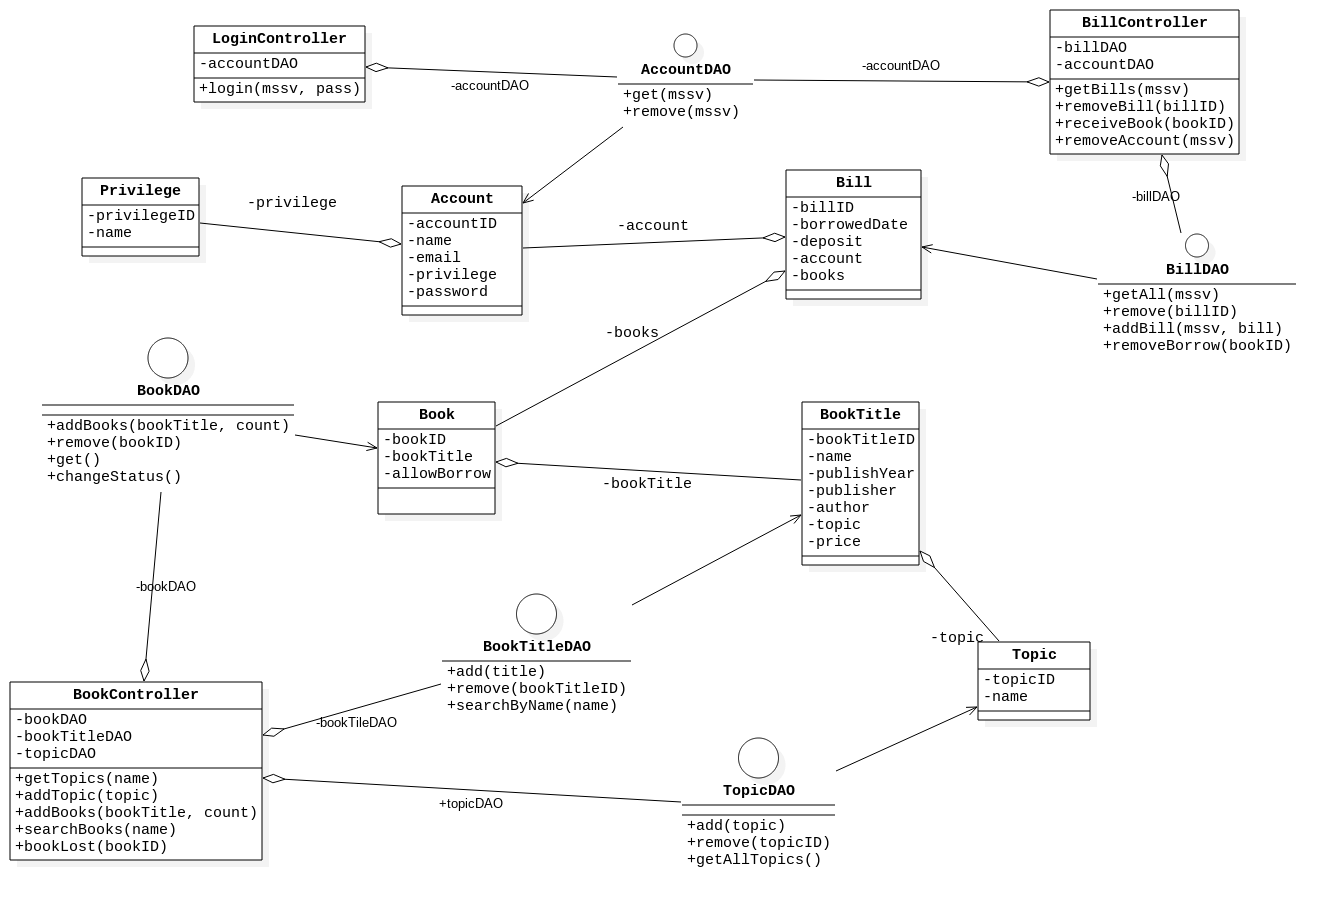
\includegraphics[width=\textwidth]{figures/class-diagram.png}
\caption{Biểu đồ lớp}
\end{figure}

% \subsection{Biểu đồ object}

\end{document}
